\documentclass{beamer}
\usepackage[spanish]{babel}
\usepackage{fontspec}
\usepackage{listings}

\usetheme{Szeged}
\usecolortheme{beaver}

\beamertemplatenavigationsymbolsempty

\title[MIPS] % (optional, only for long titles)
{M\'odulo de Identificaci\'on de Pasos y Situaciones}
\subtitle{MIPS}
\author[Rub\'en Agudo] % (optional, for multiple authors)
{Rub\'en Agudo Santos \and Mikel Villama\~ne Giron\'es}
%\institute % (optional)
%{
%	\inst{1}%
%	Alumno\\
%	Euskal Herriko Unibertsitatea (EHU)
%	\and
%	\inst{2}%
%	Director del Trabajo de Fin de Grado.\\
%	Departamento de Lenguajes y Sistemas de Informaci\'on
%}


\begin{document}
	\frame{\titlepage}
	\begin{frame}
	\frametitle{Fe de erratas}
	
	\begin{itemize}
		\item La palabra ``cont\'inuo" varias veces.
		\item La palabra ``que". P\'agina 43, p\'arrafo 1, l\'inea 1.
	\end{itemize}
\end{frame}

\begin{frame}
	\frametitle{\'Indice}
	\begin{enumerate}
		\item Antecedentes
%		\item ¿Qu\'e es MIPS?
		\item Ejemplo
		\item Desarrollo
		\item Gesti\'on
		\item Conclusiones
		\item L\'ineas futuras
	\end{enumerate}
\end{frame}

	\chapter{Antecedentes}

%Situación actual, estudio de diferentes alternativas 
%existentes o distintos posibles enfoques del problema a solucionar
\section{Situaci\'on actual}
El proyecto ULISES desarrollado por el grupo de investigaci\'on GaLan, en colaboraci\'on con la universidad de Navarra, 
consiste en un software que permite la integraci\'on de cualquier sistema interactivo con cualquier
sistema educativo. Es decir, sirve para ense\~nar habilidades que necesitan de un profesor experto que los eval\'ue,
ya sea en tiempo real, o a trav\'es de un v\'ideo.


La parte de los sistemas interactivos puede estar formada, por ejemplo, por un simulador de conducci\'on de camiones,
un sistema de captura de movimientos, un kinect, etc.

Por otro lado, el sistema educativo puede ser moodle, DETECTIVE o cualquier software que permita evaluar algo.

El objetivo principal es conseguir un sistema en el que la gente entrene una habilidad concreta, por ejemplo, aprender
a sacar correctamente en tenis, y que el sistema sea capaz de evaluar, determinar d\'onde se ha equivocado, y en definitiva,
ayudar a esa persona a aprender a realizar un saque de tenis correctamente.

Para poder realizar un diagn\'ostico, se han definido tres niveles.

\begin{enumerate}
	\item Nivel de observaci\'on
	\item Nivel de interpretaci\'on
	\item Nivel de diagn\'ostico
\end{enumerate}

\subsection{Nivel de observaci\'on}
En el nivel de observaci\'on lo que se hace es transformar los datos en bruto, 
es decir, las se\~nales y valores generados por el sistema interactivo
a los objetos que han sido definidos en el propio sistema: Observaciones y Propiedades.

Para poder determinar de manera correcta esas propiedades y observaciones, es necesario contar con un 
experto en el sistema interactivo, y un experto del dominio, que es quien define las observaciones y las
propiedades que han de tenerse en cuenta. N\'otese que el experto del dominio define las observaciones y las
propiedades en un lenguaje natural, t\'ecnico en su campo del conocimiento, pero no en el \'ambito del propio
sistema. Por su parte, el experto en el sistema interactivo es quien define
las observaciones y sus propiedades en el propio sistema
en base a los datos, valores y se\~nales que produce el sistema interactivo.

\subsubsection{Observaciones y propiedades}
Una observaci\'on representa un hecho interesante para el diagn\'ostico, y que 
adem\'as tiene sentido. Suelen
ser lo suficientemente peque\~nas para que sean f\'acilmente diagnosticables. Si la observaci\'on
fuese ``Realizar saque", ser\'ia una secuencia de varias acciones, por ejemplo: ``lanzar pelota", ``echar raqueta hacia atr\'as" \
y ``golpear pelota". De esta manera se es mucho m\'as granular y se pueden dar mejores diagn\'osticos \cite{INTRASIM:Manual}.

Cada observaci\'on contiene una serie de propiedades, que es lo que caracteriza una observaci\'on. 
Siguiendo con el ejemplo del tenis, unas posibles propiedades para la observaci\'on ``pelota en movimiento" \
pueden ser la velocidad y la direcci\'on de la pelota.

\subsection{Nivel de interpretaci\'on}
Este es un nivel clave, en el que se crean los Pasos y las Situaciones. Ambos objetos se crean en base a relaciones
entre observaciones.
Estas relaciones son necesarias, ya que no todas las observaciones que se capturan influyen en las dem\'as,
o no aportan informaci\'on \'util o relevante, y puede que incluso creen ruido, empeorando el diagn\'ostico.

\paragraph{\textbf{Paso:}}
Es el comportamiento de un conjunto de observaciones en el tiempo. Con un paso se define 
c\'omo se tienen
que comportar las observaciones y sus propiedades en un periodo de tiempo concreto. Al igual que con las observaciones,
se suelen definir pasos peque\~nos, como por ejemplo, ``levantar raqueta", para realizar los diagn\'osticos m\'as precisos.

\paragraph{\textbf{Situacion:}}
Define el contexto en el que suceden las observaciones y que influyen al Paso. Hay que
tener en cuenta que s\'olo se definen las situaciones que tienen influencia en el paso
para poder diagnosticar si lo que est\'a haciendo el alumno es correcto o no. Por ejemplo, a la hora
de tirar la pelota, habr\'ia que tener en cuenta el viento, para compensar su trayectoria. Si el alumno
tirase la pelota demasiado hacia delante, y no hay viento, eso nos indicar\'ia que est\'a realizando la acci\'on
incorrectamente. Por el contrario, si hiciese viento en contra, la acci\'on tendr\'ia un veredicto correcto
porque se est\'a lanzando hacia delante para compensar la fuerza del viento.

Actualmente, para crear las relaciones entre pasos y situaciones, hay una persona que lo realiza a mano. En muchos casos
es un trabajo de prueba y error y adem\'as con resultados sub\'optimos ya que no siempre se ven claramente las relaciones,
e incluso pueden crearse relaciones err\'oneas y que empeoren los futuros diagn\'osticos.

En esta situaci\'on es donde cobra sentido la realizaci\'on de este TFG. El software MIPS, es un primer paso para facilitar
el trabajo a la persona que crea esas relaciones. Es una herramienta de experto 
que de manera gr\'afica, permite
acotar los datos procesados en el nivel de observaci\'on. Es decir, el software no recibe datos capturados por
el sistema de realidad virtual, sino
las propiedades y observaciones, con sus valores en el tiempo durante una sesi\'on de trabajo.

Al acotar esos datos en distintos rangos se pueden definir pasos y situaciones tomando como referencia
el tiempo y los v\'ideos en caso de existir, en qu\'e momentos de la sesi\'on de trabajo
se est\'a produciendo ese paso o esa situaci\'on que se quiere definir, de manera que se obtenga
como resultado un fichero XML donde estar\'an almacenados todos los datos de aquellas observaciones y 
propiedades que el usuario haya seleccionado porque crea que son importantes para ese paso o 
situaci\'on.

Una vez creados los pasos y situaciones, se utilizar\'an algoritmos de \emph{Machine Learning} 
y miner\'ia de datos para
realizar un \emph{Feature Selection 
\footnote{\url{http://jmlr.org/papers/volume3/guyon03a/guyon03a.pdf}}},
y establecer las relaciones de manera autom\'atica.

\subsection{Nivel de diagn\'ostico}
Finalmente, en este nivel, mediante distintas t\'ecnicas de diagn\'ostico, como por ejemplo el \emph{Clustering} y
algoritmos de clasificaci\'on supervisada se determina si el alumno ha 
adquirido la habilidad. Si aun no domina lo que deseaba aprender, se le 
proporciona el \emph{feedback} 
necesario para saber donde tiene que incidir para poder mejorar.

\section{Estudio de diferentes alternativas}
Como hemos visto en la secci\'on anterior, la aplicaci\'on debe poder visualizar tanto gr\'aficos como 
v\'ideos capturados durante una sesi\'on de trabajo. Si se decide a\~nadir uno o varios v\'ideos, ir\'an
sincronizados con los gr\'aficos, para poder identificar m\'as f\'acilmente en que momentos est\'a sucediendo
algo que podr\'ia ser un paso o una situaci\'on.

Para conseguir este objetivo, se barajaron distintos tipos de acercamientos al problema.

\subsection{M\'ultiples ventanas dentro de una ventana maestra (MDI)}
La primera opci\'on barajada fue crear una interfaz MDI (Multiple Document Interface). Como ventajas se
dispon\'ia de cierta experiencia creando aplicaciones MDI en .NET.

Pero, estamos en 2014 y las ventanas MDI no son muy c\'omodas de utilizar cuando se disponen de varias ventanas
abiertas, ya que no se acoplan autom\'aticamente a los lados, ni se pueden crear pesta\~nas de manera din\'amica.
Por otro lado, las ventanas MDI fueron desaprobadas en WPF, que es el nuevo sub sistema gr\'afico para renderizar 
interfaces de usuario de Microsoft.

\subsection{Crear una interfaz tipo IDE}
La mayor\'ia de los IDEs conocidos, como Eclipse, Visual Studio, NetBeans IntelliJ Idea... disponen de un sistema de 
ventanas acoplables din\'amicas. Pueden crearse grupos de pesta\~nas, redimensionarlas, ponerlas lado a lado etc.

Debido a que el software va a desarrollarse con Visual Studio, era factible pensar que crear una interfaz similar al propio
Visual Studio ser\'ia sencillo, con controles gr\'aficos que facilitaran la tarea.

La realidad es bien distinta, ya que se necesita de componentes de terceros para crear ese tipo de interfaz. Pese a ese
peque\~no inconveniente hay distintas librer\'ias de c\'odigo abierto que proporcionan la nombrada funcionalidad.

Por tanto la alternativa que se tom\'o fue esta. Implementar una interfaz tipo IDE que permita el acoplamiento de ventanas,
crear grupos de pesta\~nas etc.
	\begin{frame}
	\frametitle{Funcionamiento actual}
	\framesubtitle{Nivel de observaci\'on}
	
	\begin{columns}[T] % contents are top vertically aligned
		\begin{column}[T]{5cm} % each column can also be its own environment
			\begin{itemize}
				\item Captura de datos
				\item Se crean
				\begin{itemize}
					\item Propiedades
					\item Observaciones
				\end{itemize}
			\end{itemize}
		\end{column}
		\begin{column}[T]{5cm} % alternative top-align that's better for graphics
			
\includegraphics[width=0.5\linewidth]{./Figures/NivelDeObservacion.png}
		\end{column}
	\end{columns}
\end{frame}

\begin{frame}
	\frametitle{Funcionamiento actual}
	\framesubtitle{Nivel de interpretaci\'on}
	
	\begin{columns}[T] % contents are top vertically aligned
		\begin{column}[T]{5cm} % each column can also be its own environment
			\begin{itemize}
				\item Relaciones entre observaciones
				\begin{itemize}
					\item Pasos
					\item Situaciones
				\end{itemize}
			\end{itemize}
		\end{column}
		\begin{column}[T]{5cm} % alternative top-align that's better for 
			%graphics
			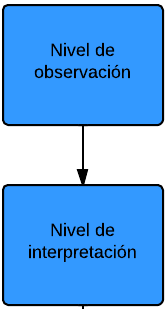
\includegraphics[width=0.5\linewidth]{./Figures/NivelDeInterpretacion.png}
		\end{column}
	\end{columns}
\end{frame}

\begin{frame}
	\frametitle{Funcionamiento actual}
	\framesubtitle{Nivel de di\'agnostico}
	
	\begin{columns}[T] % contents are top vertically aligned
		\begin{column}[T]{5cm} % each column can also be its own environment
			\begin{itemize}
				\item Usando distintos m\'etodos de diagn\'ostico
				\begin{itemize}
					\item \textit{Clustering}
					\item Clasificaci\'on supervisada
					\item ...
				\end{itemize}
			\end{itemize}
		\end{column}
		\begin{column}[T]{5cm} % alternative top-align that's better for 
			%graphics
			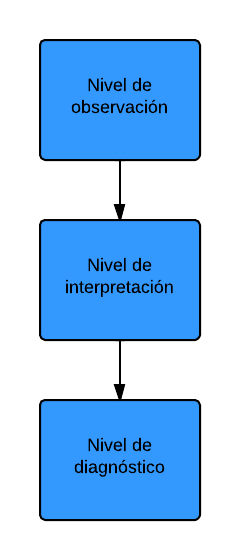
\includegraphics[width=0.5\linewidth]{./Figures/NivelDeDiagnostico.png}
		\end{column}
	\end{columns}
\end{frame}
	\begin{frame}
	\frametitle{Despu\'es del proyecto}
	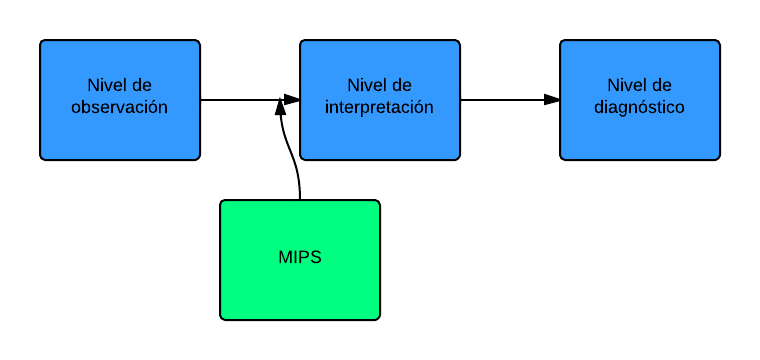
\includegraphics[width=1.0\linewidth]{./Figures/DespuesDelProyecto.png}
	
\end{frame}
	%\section{¿Qu\'e es MIPS?}
\begin{frame}
	\frametitle{¿Qu\'e es MIPS?}
	
	\begin{itemize}
		\item Herramienta de autor para el experto
		\item Permite
		\begin{itemize}
			\item Selecci\'on de rangos
			\item Ayuda la identificaci\'on de pasos y situaciones
			\item Exportar esos rangos
		\end{itemize}
	\end{itemize}
\end{frame}

%\section{¿Por qu\'e es necesario?}
\begin{frame}
	\frametitle{¿Por qu\'e es necesario?}
	
	\begin{itemize}
		\item Identificaci\'on manual de pasos y situaciones
		\item Prueba y error
		\item Relaciones err\'oneas
		\item Resultados sub\'optimos
	\end{itemize}
\end{frame}
	\begin{frame}
	\frametitle{¿Por qu\'e es necesario?}
	
	\begin{itemize}
		\item Identificaci\'on manual de pasos y situaciones
		\item Prueba y error
		\item Relaciones err\'oneas
		\item Resultados sub\'optimos
	\end{itemize}
\end{frame}
	\begin{frame}
	\frametitle{Ejemplo de observaciones y propiedades}
	
	\begin{columns}[T] % contents are top vertically aligned
		\begin{column}[T]{5cm} % each column can also be its own environment
			\begin{center}
				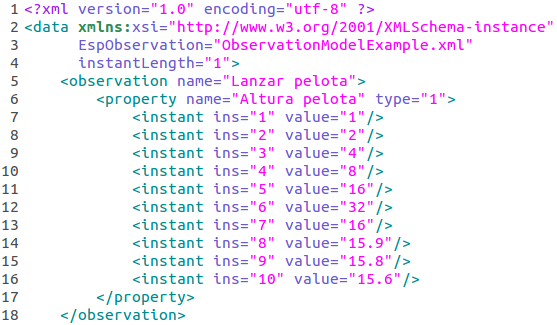
\includegraphics[width=1.1\linewidth]{./Figures/Datos1.png}
			\end{center}

		\end{column}
		\begin{column}[T]{5cm} % alternative top-align that's better for 
			\begin{center}
				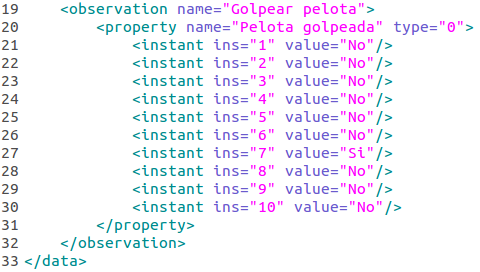
\includegraphics[width=1.1\linewidth]{./Figures/Datos2.png}
			\end{center}
		\end{column}
	\end{columns}
\end{frame}
	\begin{frame}
	\frametitle{Ejemplo de visualizaci\'on en MIPS}
	\begin{center}
		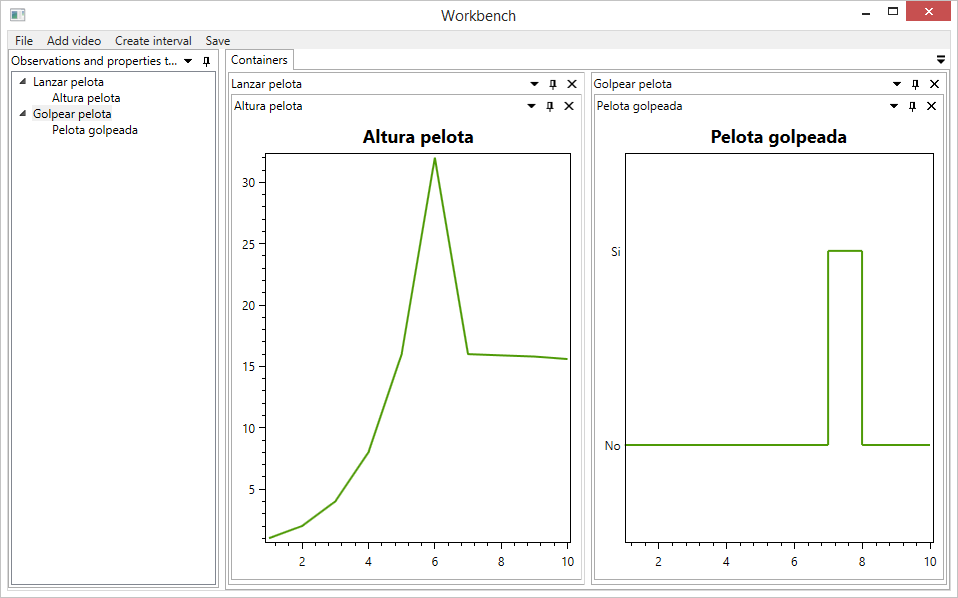
\includegraphics[width=1.0\linewidth]{./Figures/EjemploObservacion.PNG}
	\end{center}
\end{frame}
	%\section{Herramientas utilizadas}
\begin{frame}
	\frametitle{Desarrollo}
	\framesubtitle{Herramientas utilizadas}
	
	\begin{itemize}
		\item Visual Studio 2013 Ultimate
		\item OxyPlot
		\item AvalonDock
		\item Git
		\item \LaTeX \ y TeXstudio
	\end{itemize}
\end{frame}

\begin{frame}
	\frametitle{Dise\~no}
	\framesubtitle{SOLID y patrones}
	\begin{columns}[T]
		
		\begin{column}[T]{0.5\linewidth}
			\begin{block}{SOLID}
				\begin{itemize}
					\item \textbf{S}ingle responsibility principle
					\item \textbf{O}pen-closed principle
					\item \textbf{L}iskov substitution principle
					\item \textbf{I}nterface segregation principle
					\item \textbf{D}ependency inversion principle
				\end{itemize}
			\end{block}
		\end{column}
		
		\begin{column}[T]{0.5\linewidth}
			\begin{block}{Patrones}
				\begin{itemize}
					\item Model View View-Model
					\item Iterator
					\item Singleton
				\end{itemize}
			\end{block}
		\end{column}
		
	\end{columns}

\end{frame}

%\section{Desarrollo}
\begin{frame}
	\frametitle{Desarrollo}
	\framesubtitle{Qu\'e se ha hecho}
	Una aplicaci\'on que permite:
	\begin{enumerate}
		\item Cargar un XML con las observaciones y propiedades
		\item Visualizar datos discretos y continuos
		\item Cargar v\'ideos y visualizarlos
		\item Seleccionar rangos
		\item Exportar los rangos seleccionados en XML
		\item Organizar los elementos como se desee, tipo Eclipse o Visual 
		Studio
	\end{enumerate}
	
\end{frame}



	\begin{frame}
	\frametitle{Herramientas utilizadas}
	
	\begin{itemize}
		\item Visual Studio 2013 Ultimate
		\item OxyPlot
		\item AvalonDock
		\item GVim
		\item \LaTeX y TeXstudio
	\end{itemize}
\end{frame}
	%\section{Gesti\'on}
\begin{frame}
	\frametitle{Gesti\'on}
	
	\begin{itemize}
		\item Se han utilizado metodolog\'ias \'agiles de desarrollo
		\begin{itemize}
			\item Scrum
			\item Kanban
		\end{itemize}
	\end{itemize}
	
\end{frame}

%\subsection{Scrum}
%\begin{frame}
%	\frametitle{Gesti\'on}
%	\framesubtitle{Scrum: ¿Qu\'e es?}
%	\begin{columns}[T] % contents are top vertically aligned
%		
%		\begin{column}[T]{0.5\linewidth} % each column can also be its own 
%			\textbf{¿Qu\'e es?}
%			\begin{itemize}
%				\item M\'etodo de desarrollo iterativo e incremental
%				\item En cada ciclo de desarrollo (sprint) se genera un 
%				entregable.
%				\item Lo importante es que el diferencial de valor incremente
%			\end{itemize}
%		\end{column}
%		\begin{column}[T]{0.5\linewidth} % alternative top-align that's better 
%			%for graphics
%			\begin{figure}
%				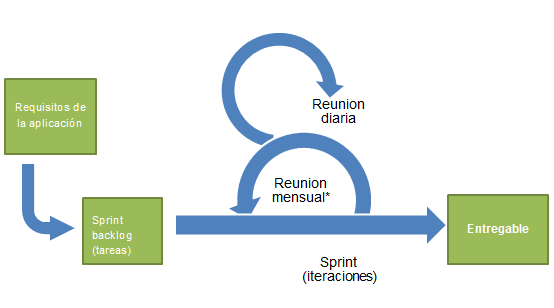
\includegraphics[width=1.0\linewidth]{./Figures/Scrumm.PNG}
%				\label{scrum}
%			\end{figure}
%			
%\tiny{\url{https://upload.wikimedia.org/wikipedia/commons/e/e5/Scrumm.PNG}
%					
%					Autor: Maxie Ayala 
%					Licenciado bajo 
%					\hyperlink{creativecommons.org/licenses/by-sa/3.0/}{CC 
%					BY-SA 3.0}}
%		\end{column}
%	\end{columns}
%
%\end{frame}
%
%%\subsection{Kanban}
%\begin{frame}
%	\frametitle{Gesti\'on}
%	\framesubtitle{Kanban: ¿Qu\'e es?}
%	
%	\textbf{¿Qu\'e es?}
%	\begin{itemize}
%		\item M\'etodo de gesti\'on del trabajo que se est\'a realizando
%		\item T\'ipicamente se utiliza un tablero o corcho con 3 columnas
%		\item Por columnas, m\'inimo se suele poner:
%		\begin{enumerate}
%			\item Qu\'e est\'a pendiente por hacer
%			\item Qu\'e se est\'a haciendo actualmente
%			\item Qu\'e se ha terminado
%		\end{enumerate}
%		
%	\end{itemize}
%	
%	
%\end{frame}

\begin{frame}
	\frametitle{Gesti\'on}
	\framesubtitle{Scrum: C\'omo se ha usado}
	
	\textbf{Ha habido 7 sprints, de un mes de duraci\'on}
	\begin{enumerate}
		\item Se ha creado un listado de tareas (Scrum backlog)
		\item Se han ordenado las tareas por prioridad
		\item Por cada sprint
		\begin{enumerate}
			\item Se seleccionan m\'aximo 3 tareas por sprint (Sprint backlog)
			\item Se desarrollan las funcionalidades
			\item Se documentan
			\item Se despliega
		\end{enumerate}
	\end{enumerate}	
\end{frame}

\begin{frame}
	\frametitle{Gesti\'on}
	\framesubtitle{Kanban: C\'omo se ha usado}
	\begin{itemize}
		\item Columna ``Por hacer": Scrum backlog
		\item Columna ``En progreso": Sprint backlog
		\item Columna ``Finalizado": Tareas finalizadas organizadas por 
		sprint
	\end{itemize}
\end{frame}
	\begin{frame}
	\frametitle{Conclusiones}
	\framesubtitle{Sobre la gesti\'on}
	
	\begin{columns}[T] % contents are top vertically aligned
		
		\begin{column}[T]{0.35\linewidth} % each column can also be its own 
			%environment
			\begin{itemize}
				\item Ha habido retraso
				\item Para mitigarlo
				\begin{itemize}
					\item Scrum
					\item Kanban
					\item Meter m\'as horas
				\end{itemize}
			\end{itemize}
		\end{column}
		
		\begin{column}[T]{0.65\linewidth} % alternative top-align that's better 
			%for graphics
			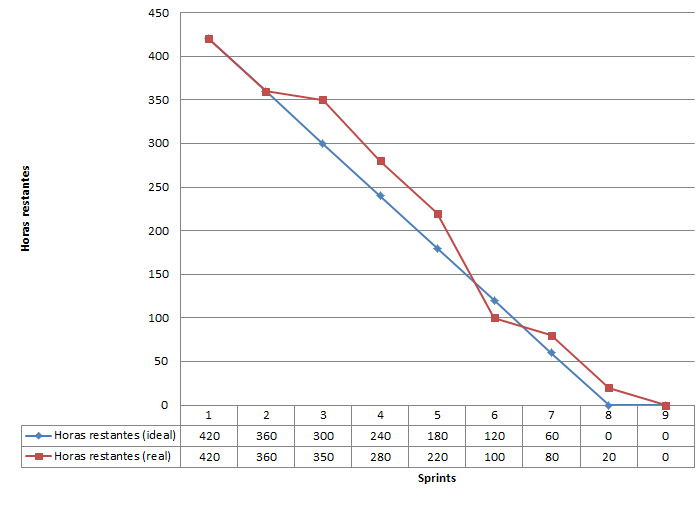
\includegraphics[width=1.0\linewidth]{./Figures/burndown.png}
		\end{column}
	\end{columns}
\end{frame}

\begin{frame}
	\frametitle{Conclusiones}
	\framesubtitle{Personales}
	
	\begin{itemize}
		\item S\'indrome del programador
		\item Dif\'icil programar sin documentaci\'on
		\item Estar fuera de la zona de ``confort"
	\end{itemize}
\end{frame}


	\begin{frame}
	\frametitle{L\'ineas futuras}
	\framesubtitle{Mejoras}
	Ordenadas de m\'as importante a menos importante
	\begin{enumerate}
		\item Que el software sea m\'as abstracto
		\item Utilizar Desarrollo Dirigido por Pruebas (Test Driven Development)
		\item Mejorar el procesamiento paralelo.
		\item Eliminar Singleton por patrones Factory
		\item Utilizar los \emph{data bindings} de MVVM
	\end{enumerate}
	\textbf{Refactorizar, refactorizar, refactorizar}
\end{frame}
\end{document}
